\documentclass{article}
\usepackage[margin=1in]{geometry}
\usepackage{mathtools, amsfonts, amsthm, xcolor}

\title{Title}
\author{Your name here}

\begin{document}
\maketitle

\section*{Exercise 1 [2]}

Collaborators: Jared Contreras
\\
Tools and resources used: On Exercise 1, I used ChatGPT to help me figure out how to [...]. On Choice Exercise 7, I watched a YouTube video to [...].
\\
\begin{enumerate}
  \item[Exercise 1]
    {\color{red} Points attempted: 2}.
    {\color{blue} Time spent: 5 minutes}.
    {\color{brown} Difficulty: 1/10}.
    {\color{green!50!black} Self-assessed score: 2}.
    {\color{magenta} Questions/Feedback: None.}
  \item[Exercise 2]
    {\color{red} Points attempted: 1}.
    {\color{blue} Time spent: 2 minutes}.
    {\color{brown} Difficulty: 1/10}.
    {\color{green!50!black} Self-assessed score: 1}.
    {\color{magenta} Questions/Feedback: None.}
  \item[Exercise 3]
    {\color{red} Points attempted: 6}.
    {\color{blue} Time spent: 30 minutes}.
    {\color{brown} Difficulty: 3/10}.
    {\color{green!50!black} Self-assessed score: 6}.
    {\color{magenta} Questions/Feedback: Did I do the problem correctly and as intended?}
\end{enumerate}

\section*{Exercise 2 [1]}

Done! Posted an image of a marker with rotational symmetry.

\section*{Exercise 3 [6]}
\begin{enumerate}
    \item { 
        The coins have 8 symmetries. That is because there are \(2^2\) configurations 
        without swapping places. When allowing swapping places, we get \(2 \times 2^2 = 8\).
    }
    \item {
        First, I chose the symmetry of flipping the \emph{left}, denoted as \(f_L\), 
        coin over. Applying 
        this symmetry twice gets us back to id. However, when we allow the swapping 
        of places, denoted \(s\), we can actually get to all states. 
        We do not actually need an explicit `flip right' symmetry, since it is 
        actually equal to \(f_L \circ s\).
    }
    \item {
        In the diagram, let \(a=f_L\) and \(b=s\).

        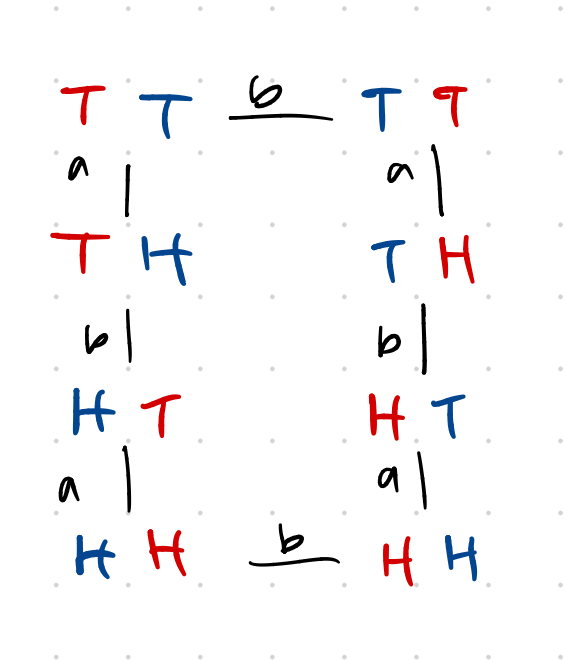
\includegraphics[width=\linewidth]{ex3.png}
    }
    \item {
        I used 2 generators.
    }
    \item {
        This group is not commutative. This is because \(f_L \circ s \not= s \circ f_L\). 
        Swapping the coins then flipping the left is not the same as flipping 
        then swapping.
    }
\end{enumerate}
\end{document}
